\documentclass[a4paper]{report}
\usepackage{times}
\usepackage[utf8]{inputenc}
\usepackage[pdftex]{graphicx}
\usepackage{multicol}

% to customize headers and footers
\usepackage{fancyhdr}
\pagestyle{fancy}
\chead{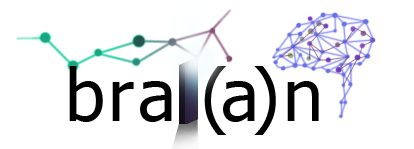
\includegraphics[scale=0.2]{braian}}
\rfoot{\vspace{1cm} 
\includegraphics[scale=0.03]{Logo-Epitech}}

\newcommand{\HRule}{\rule{\linewidth}{0.5mm}}

\begin{document}
  \begin{titlepage}
  \begin{center}

    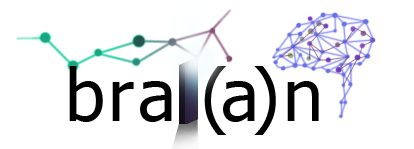
\includegraphics[width=0.7\textwidth]{braian}~\\[1cm]

    \textsc{\LARGE Epitech Paris}\\[1.5cm]

    \textsc{\Large Fiche Projet - PFA}\\[0.5cm]

    % Title
    \HRule \\[0.4cm]
    { \huge \bfseries Brai(a)n - An AI who learns \\[0.4cm] }

    \HRule \\[1.5cm]

    \noindent

    \begin{multicols}{3}
      \emph{Chef Technique:}\\
      Sebastien \textsc{Maire} \\

      \vspace{1cm}

      \emph{Technique:} \\
      Alexandre \textsc{Fulgoni} \\

      \emph{Technique:} \\
      Stephane \textsc{Nguyen} \\

      \vspace{1cm}

      \emph{Manageur:} \\
      Thomas \textsc{Nieto} \\

      \vspace{1cm}

      \emph{Technique:} \\
      Emmanuel \textsc{Isidore} \\

      \vspace{1cm}

      \emph{Technique:} \\
      Thomas \textsc{Valentin} \\
   \end{multicols}

    \vfill

    {\large \today}

  \end{center}

  \begin{flushright}
    \vspace{1cm}
    
\includegraphics[scale=0.03]{Logo-Epitech}
  \end{flushright}

\end{titlepage}



  \section{Introduction}
  Au regard de ce que la science-fiction a imaginé dans le domaine de l'intelligence artificielle, l'informatique moderne n'en est qu'à ses balbutiements.
  Prenons quelques examples en littérature : HAL dans 2001, l'Odyssée de l'Espace ;
  en cinéma : JARVIS dans Iron-Man ou Mr. Smith dans Matrix ; ou encore dans le jeu-vidéo : Cortana dans HALO... Pour ne citer qu'eux. \\
  Le plus pertinant exemple d'IA qui nous accompagne ? Siri, une voix monotone dans un téléphone qui se décharge en dix heures...
  D'une part, nous avons de vraies personnages et d'autre part, une assistante électronique aux réponses hasardeuses.

  \noindent
  La différence la plus flagrante entre ces IA et Siri ? Leur comportement. \\
  En effet, le cadre de la science-fiction permet tous les possibles. Les IA qui en sont issues évoluent, intéragissent, échangent, se remettent en question.
  Seulement, cela n'est permis qu'avec la faculté d'appendre. Quid de l'apprentissage dans l'IA réelle ? \\

  \noindent
  C'est sur ce dernier point, que nous avons décidé de travailler. \\
  Nous nous concentrerons alors, sur l'aspect apprentissage et la prise de décision d'une intelligence artificielle.

  \section{Equipe}
    \begin{description}
      \item[Sébastien Maire] \hfill \\
        \textbf{Chef Technique} \\
        Motivé par l'application de ses connaîssances en algorithmie et leur approndissement
      \item[Alexandre Fulgoni] \hfill \\
        \textbf{technique} \\
        A toujours été motivé par l'IA et leurs domaines d'application.
      \item[Stéphane Nguyen] \hfill \\
        \textbf{technique} \\
        intéressé par le développement de jeu-vidéo. En effet,
        au-delà du graphisme, l’IA est LE pillier qui permet le réalisme
        et donc l’immersion du joueur.
      \item[Thomas Nieto] \hfill \\
        \textbf{Recherche et management} \\
        Curieux de tout et motivé.
    \end{description}

  \noindent
  Première fois ensemble dans un groupe. Nous nous sommes rencontrés grâce aux
  intérêts que nous partageons et sommes donc tous motivés pour aller le plus
  loin possible.

  \section{Contexte}
  Afin de tester les différentes versions de nos intelligences artificielles, nous allons nous servir d'environnements virtuels ouverts (dit sandbox).
  Ces derniers permettront de disposer de tous les éléments qui structurent notre monde, mais dans une version simpliste et programmable.
  Nous pensons, alors, utiliser les mécanismes de cycles de vies, de gravité, de faim, ainsi que les diverses interactations sociales, etc.

  \section{Partenaire}

  L'Epitech Innovation HUB en la personne de Thibaut Royer.

  \section{Objectifs}
  Dans un premier temps, nous voulons implémenter un système complet de prise de décision dont les noeuds seraient capable de se rééquilibrer. Le but est
  de mettre en place un système capable de s'adapter à plusieurs situations. Pour aller plus loin, nous voudrions être capable de mettre en place
  une intelligence articielle capable d'intégrer à son arbre de décision, de nouveaux noeuds.
  Coupler prise de décision et apprentissage
  Cas concret : arbre de décision qui change ses nodes.

  \section{Planning}
  2 jours par semaine : Samedi et dimanche

\end{document}
